\documentclass{article}
\usepackage{mathrsfs}
\usepackage{harpoon}
\usepackage{comment}
\usepackage{color}
\usepackage{amsmath}
\usepackage{amssymb}
\usepackage{mathtools}
\usepackage{simplewick} 
\usepackage{graphicx} % added for subfig
\usepackage{subfigure} % added for subfig
\usepackage{physics}
\usepackage{amssymb}
\usepackage{slashed}

\title{Matching kernel in the coordinate space for pion DA}
\author{Jinchen He}
\date{}
\usepackage[a4paper,left=20mm,right=20mm,top=20mm,bottom=20mm]{geometry}
\begin{document}
\maketitle
%\tableofcontents
%\pagebreak[4]

\section{Theoretical deduction by Fei Yao}

The light-cone pion distribution amplitude

\begin{equation}
	q(x)=\int \frac{dz^-}{2\pi} e^{-ix p^+ z^-}  \langle \pi(p)|\bar{\psi}(z)  \gamma^{+} \gamma^{5} L(z,0) \psi(0)|0 \rangle
\end{equation}
 
Light-cone amplitude can be studied from the large momentum limit of the following quasi correlation

\begin{equation}
	\tilde{q}(x,p^z)=\int \frac{dz}{2\pi} e^{ix p^z z} \langle \pi(p)|\bar{\psi}(\text{z})  \gamma^{z} \gamma^{5}  L(z,0) \psi(0)|0 \rangle
\end{equation}

where $\text{z}=(0,0,0,z),\zeta=zp_z$, the connection between these two quantities  is given by the following factorization formula

\begin{equation}
   \tilde{q}(x,p^z,\mu)= \int_{0}^{1} dy C(x,y,\mu,p^z) q(y,\mu)
\end{equation}

where the factor C depends on UV physics only.

\phantom{}

the coordinate space correlation

\begin{equation}
	\tilde{M}(x\zeta,\mu^2 z^2 )=\langle \pi(p)|\bar{\psi}(\text{z})  \gamma^{z} \gamma^{5}  L(z,0) \psi(0)|0 \rangle
\end{equation}

\phantom{}

At first, we need to compute the coordinate space correlation perturbatively. at tree level

\begin{equation}
	 \tilde{M}^{(0)}=\bar{u}(p_1)\gamma^z \gamma_5 v(p_2) e^{-izp_{1z}}
\end{equation}


At one-loop level, the contributing diagrams are depicted in Fig.1.

\begin{figure}
 	\centering
 	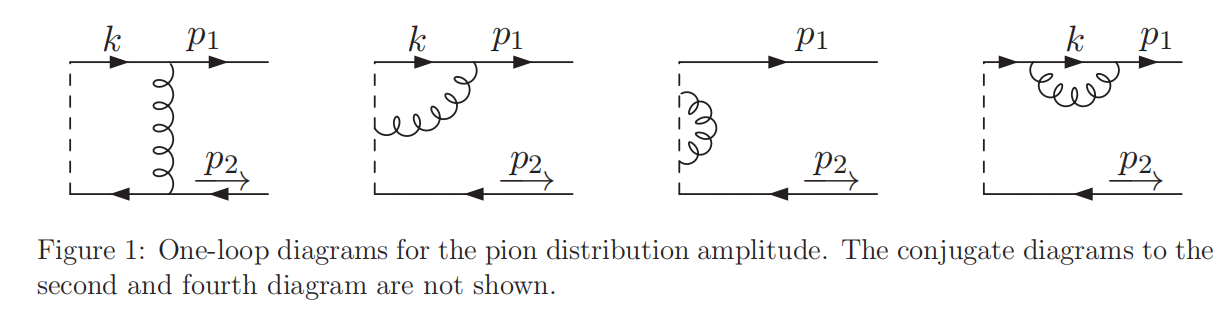
\includegraphics[scale=0.7]{fig1.png} 	
\end{figure} 

   
\begin{align}{}
	&\tilde{\Gamma}_1 =\int \frac{d^4 k}{(2\pi)^4}\bar{u}(p_1)(-i g t^a \gamma^\mu) \frac{i}{\slashed{k}} \slashed{\text{z}} \gamma_5 \frac{i}{\slashed{k}-\slashed{p_1}-\slashed{p_2}} (-i g t^a \gamma_\mu) \frac{-i}{(p_1-k)^2} v(p_2) e^{ik\cdot \text{z}}\notag\\		
	&\quad=-i g^2 C_F  \int \frac{d^4 k}{(2\pi)^4}\bar{u}(p_1) \frac{1}{k^2 (k-p)^2 (p_1-k)^2}[\gamma^\mu \slashed{k} \slashed{\text{z}} \gamma_5 (\slashed{k}-\slashed{p})\gamma_\mu] v(p_2) e^{ik\cdot \text{z}} \notag\\
	&\quad=-i g^2 C_F \int \frac{d^4 k}{(2\pi)^4}\bar{u}(p_1) \frac{1}{(p_1-k)^2 (k+p_2)^2 k^2}[\gamma^\mu (\slashed{p_1}-\slashed{k}) \slashed{\text{z}} \gamma_5 (-\slashed{p_2}-\slashed{k})\gamma_\mu] v(p_2) e^{i(p_1-k)\cdot \text{z}}\notag\\
	&\quad= -i g^2 C_F  e^{ip_1\cdot \text{z}} \int \frac{d^4 k}{(2\pi)^4}\bar{u}(p_1) \int_{0}^{1} dx dy \frac{2 \bar{y}}{[(k+yp_2-(1-y)xp_1)^2]^3}[\gamma^\mu (p_1-i\partial_\text{z})_\rho \gamma^\rho \slashed{\text{z}} \gamma_5\notag\\
	& \qquad (-p_2-i\partial_\text{z})_\sigma \gamma^\sigma \gamma_\mu] v(p_2) e^{-i k \cdot \text{z}}\notag\\
	&\quad= -i g^2 C_F  \mu^{2\epsilon} e^{ip_1\cdot \text{z}} \bar{u}(p_1) \int_{0}^{1} dx dy 2\bar{y} [\gamma^\mu \gamma^\rho \slashed{\text{z}} \gamma_5 \gamma^\sigma \gamma_\mu] (p_1-i\partial_z)_\rho (-p_2-i\partial_z)_\sigma \int \frac{d^D k}{(2\pi)^D} \frac{e^{-i k \cdot \text{z}}}{[k^2]^3}\notag\\ 
	&\qquad e^{-i((1-y)xp_1-yp_2)\cdot \text{z}}  v(p_2) \notag\\
   &\quad= \frac{\alpha_s C_F}{2\pi} \bar{u}(p_1) \slashed{\text{z}} \gamma_5 v(p_2) (\mu^2z^2\pi)^\epsilon \frac{\Gamma(2-\epsilon)}{\epsilon} (2\epsilon-1) \frac{x(e^{-i\zeta}-1)-e^{-ix\zeta}+1}{(x-1)x\zeta^2} \notag\\
\end{align}

  
where $p^\mu=p_1^\mu+p_2^\mu$, $p_1^\mu=xp^\mu$. we have chosen dimensional regularization $(D = 4 -2 \epsilon )$ for the UV divergences to simplify
the computation of momentum integrals. In the calculation, $\epsilon_{UV}$ and $\epsilon_{IR}$ are not distinguished, so there is no need to calculate the oneloop light-cone correlation function.
    
    \phantom{}
    
The second diagram and its conjugate diagram 
    
      
  \begin{align}{}
 	&\tilde{\Gamma}_{21}=\bar{u}(p_1)(-igt^a\gamma^\mu) \int \frac{d^4 k}{(2\pi)^4} \frac{1}{\slashed{k}} \slashed{\text{z}} \gamma_5 (-i g t^a)\int_{0}^{1} du \text{z}_\mu \frac{-i}{(p_1-k)^2}e^{ik\cdot \text{z}+ iu (p_1-k)\cdot \text{z}}v(p_2)\notag\\
 	& \quad =-g^2 C_F \bar{u}(p_1) \int_{0}^{1} du \int \frac{d^4 k}{(2\pi)^4} \frac{\slashed{\text{z}}\slashed{k}\slashed{\text{z}} \gamma_5}{k^2(p_1-k)^2}e^{i\bar{u} k\cdot\text{z}+ i u p_1 \cdot \text{z}}v(p_2)\notag\\
 	& \quad =-g^2 C_F \bar{u}(p_1)\int_{0}^{1} du \int \frac{d^4 k}{(2\pi)^4} \frac{\slashed{\text{z}}(\slashed{p_1}-\slashed{k})\slashed{\text{z}} \gamma_5}{k^2(p_1-k)^2}e^{ip_1\cdot \text{z}-i\bar{u}k\cdot\text{z}}v(p_2)\notag\\	
 	& \quad =-g^2 C_F \bar{u}(p_1)\int_{0}^{1} du \int \frac{d^4 k}{(2\pi)^4} \frac{\slashed{\text{z}}(\slashed{p_1}-\slashed{k})\slashed{\text{z}} \gamma_5}{k^2(p_1-k)^2}e^{ip_1\cdot \text{z}-i\bar{u}k\cdot z}v(p_2)\notag\\	
    & \quad =\frac{\alpha_s C_F}{2\pi} \Gamma(-\epsilon)(z^2\mu^2)^\epsilon \pi^\epsilon \int_{0}^{1}d\alpha (\frac{1-\epsilon}{1-2\epsilon}\frac{1}{\alpha} (\alpha^{2\epsilon}-\alpha)e^{-i \alpha p_1 \cdot \text{z}}-\frac{1}{2\epsilon})e^{i p_1 \cdot \text{z}} \bar{u}(p_1) \slashed{\text{z}} \gamma_5 v(p_2)\notag\\		
    & \quad =\frac{\alpha_s C_F}{2\pi} \frac{\Gamma(1-\epsilon)}{-\epsilon} (z^2\mu^2)^\epsilon \pi^\epsilon \big\{\frac{1-\epsilon}{1-2\epsilon}[(-i x\zeta)^{-2\epsilon}(\Gamma(2\epsilon)-\Gamma(2\epsilon,-i x\zeta))+\frac{e^{i \zeta}-1}{-ix\zeta}]-\frac{1}{2\epsilon}\big\}e^{-ix\zeta}\notag\\
    &\qquad \times \bar{u}(p_1) \slashed{\text{z}} \gamma_5 v(p_2)\notag\\	
   \end{align}

  
     \begin{align}{}
   	&\tilde{\Gamma}_{22} =\frac{\alpha_s C_F}{2\pi} \Gamma(-\epsilon)(z^2\mu^2)^\epsilon \pi^\epsilon \int_{0}^{1}d\alpha (\frac{1-\epsilon}{1-2\epsilon}\frac{1}{\alpha} (\alpha^{2\epsilon}-\alpha)e^{i \alpha p_2 \cdot \text{z}}-\frac{1}{2\epsilon})e^{i p_1 \cdot \text{z}} \bar{u}(p_1) \slashed{\text{z}} \gamma_5 v(p_2)\notag\\		
   	& \quad =\frac{\alpha_s C_F}{2\pi} \frac{\Gamma(1-\epsilon)}{-\epsilon} (z^2\mu^2)^\epsilon \pi^\epsilon \big\{\frac{1-\epsilon}{1-2\epsilon}[(i (1-x)\zeta)^{-2\epsilon}(\Gamma(2\epsilon)-\Gamma(2\epsilon,i(1-x)\zeta))+\frac{1-e^{-i (1-x)\zeta}}{-i(1-x)\zeta}]\notag\\
   	& \qquad-\frac{1}{2\epsilon}\big\}e^{-ix\zeta} \times \bar{u}(p_1) \slashed{\text{z}} \gamma_5 v(p_2)\notag\\	
   \end{align}
  
  The third diagram yields

    \begin{align}{}
    &\tilde{\Gamma}_3=-g^2 C_F\bar{u}(p_1) e^{i z \cdot p_1} \slashed{\text{z}} \gamma_5 \int_{0}^{1} du_1 \int_{0}^{u_1} du_2 \frac{4 \Gamma(-\epsilon) (-\text{z}^2)^\epsilon}{(4\pi)^{\frac{d}{2}}}(u_1-u_2)^{2\epsilon-2} v(p_2)\notag\\
 	&\quad =\frac{\alpha_s C_F}{2\pi} (\mu^2 z^2 \pi)^\epsilon \frac{\Gamma(1-\epsilon)}{\epsilon(1-2\epsilon)}e^{-ix\zeta} \bar{u}(p_1) \slashed{\text{z}} \gamma_5 v(p_2)\notag\\
    \end{align}


\subsection{Matching coefficient in coordinate space}

\begin{align}{}
    \tilde{M}^{(1)}(x,y,\mu^2 z^2)=&\frac{\alpha_s C_F}{2\pi} \int_{0}^{1} dx dy \theta(1-x-y)\big\{-\big(\text{ln}z^2\mu^2+\text{ln}\frac{e^{2 \gamma_E}}{4}+1\big)\big(1+\big(\frac{\bar{x}}{x}\big)_+\delta(y)\notag\\
    &+\big(\frac{\bar{y}}{y}\big)_+\delta(x)-2\delta(x)\delta(y)\big)+4-2\big(\frac{\text{ln}x}{x}\big)_+\delta(y)-2\big(\frac{\text{ln}y}{y}\big)_+\delta(x)\big\}e^{i(x-1)z p_{1z}-iyz p_{2z}}
\end{align}

After renormalizing the UV divergences in the distribution amplitudes in the $\overline{MS}$ scheme, the matching condition can be written as

\begin{align}{}
        \tilde{M}(z,0)=\int_{0}^{1} dxdy\theta(1-x-y) Z(x,y,z^2\mu^2) M((x-1)z,yz)
\end{align}


 \begin{align}{}
 Z^{(1)}(x,y,z^2\mu^2)=&\frac{\alpha_s C_F}{2\pi}\big\{-\big(\text{ln}z^2\mu^2+\text{ln}\frac{e^{2 \gamma_E}}{4}+1\big)\big(1+\big(\frac{\bar{x}}{x}\big)_+\delta(y)+\big(\frac{\bar{y}}{y}\big)_+\delta(x)-2\delta(x)\delta(y)\big)\notag\\
 &+4-2\big(\frac{\text{ln}x}{x}\big)_+\delta(y)-2\big(\frac{\text{ln}y}{y}\big)_+\delta(x)\big\}
\end{align}

Spatial correlation function of zero momentum


\begin{align}{}
    &\tilde{\Gamma}(\zeta=0) =\frac{\alpha_s C_F}{2\pi} (\frac{3}{2}(\frac{1}{\epsilon}+ln z^2\mu^2+\gamma_E +ln\pi)+\frac{7}{2})\notag\\
    &\tilde{\Gamma}_{\overline{MS}}(\zeta=0) =\frac{\alpha_s C_F}{2\pi} (\frac{3}{2}(ln z^2\mu^2+ln\frac{e^{2\gamma_E}}{4})+\frac{7}{2})\notag\\	
\end{align} 

\subsection{Pseudo-DA and matching coefficient}

\begin{align}{}
    &\tilde{M}(x\zeta,\mu^2 z^2)=\frac{\alpha_s C_F}{2\pi} (\mu^2 z^2 \pi)^\epsilon \bar{u}(p_1) \slashed{\text{z}} \gamma_5 v(p_2) \frac{\Gamma(2-\epsilon)}{-\epsilon} \bigg\{ (1-2\epsilon) \frac{x(e^{-i\zeta}-1)-e^{-ix\zeta}+1}{(x-1)x\zeta^2}\notag\\
    &\quad +\frac{1}{1-2\epsilon}\big[ (-i x\zeta)^{-2\epsilon}(\Gamma(2\epsilon)-\Gamma(2\epsilon,-i x\zeta))+\frac{e^{i \zeta}-1}{-ix\zeta}+(i (1-x)\zeta)^{-2\epsilon}(\Gamma(2\epsilon)-\Gamma(2\epsilon,i(1-x)\zeta))\notag\\
    & \quad +\frac{1-e^{-i (1-x)\zeta}}{-i(1-x)\zeta}-\frac{1}{\epsilon}  \big]e^{-i x \zeta}  \bigg \} \notag\\
\end{align}


The pseudo-DA is the Fourier transform of the spatial correlator. 

\begin{equation}
   \mathcal{P}(x,y,\mu^2z^2)= \int_{-\infty}^{\infty} \frac{d\zeta}{2\pi}e^{iy\zeta}\tilde{M}(x,\zeta,\mu^2 z^2)
\end{equation}

factorization formula for pseudo-DA

\begin{equation}
   \mathcal{P}(y,\mu^2z^2)= \int_{0}^{1} dx	\mathcal{C}(x,y,\mu^2z^2) q(x,\mu)
\end{equation}

the matching coefficient relating the pseudo-DA and light-cone DA in the $\overline{MS}$ scheme is

\begin{align}
	\mathcal{C}_{\overline{MS}}(x,y,\mu^2z^2)&= \delta(y-x)+\frac{\alpha_s C_F}{2\pi}\begin{cases}
		\qty[h(x,y,\mu^2z^2)]_{+(x)} & 0<y<x \\
		\qty[h(1-x,1-y,\mu^2z^2)]_{+(x)} & x<y<1  \notag
	\end{cases}\notag\\ & + \frac{\alpha_s C_F}{2\pi} (\frac{3}{2}(ln z^2\mu^2+ln\dfrac{e^{2\gamma_E}}{4})+\frac{7}{2})\delta(y-x) \notag
    \end{align}

\begin{equation}
	h(x,y,\mu^2z^2)= \frac{y}{x}\frac{1+x-y}{x-y}(-ln(\mu^2 z^2)-ln\frac{e^{2\gamma_E}}{4}-1)+4\frac{y}{x}+\frac{2}{x-y}ln\frac{x}{x-y}
\end{equation}

the matching coefficient relating the pseudo-DA and light-cone DA in the ratio scheme is
  
     \begin{align}
  	\mathcal{C}_{ratio}(x,y,\mu^2z^2)&= \delta(y-x)+\frac{\alpha_s C_F}{2\pi}\begin{cases}
  		\qty[h(x,y,\mu^2z^2)]_{+(x)} & 0<y<x \\
  		\qty[h(1-x,1-y,\mu^2z^2)]_{+(x)} & x<y<1  \notag
  	\end{cases}\notag
  \end{align}
  
  \begin{equation}
  	h(x,y,\mu^2z^2)= \frac{y}{x}\frac{1+x-y}{x-y}(-ln(\mu^2 z^2)-ln(\frac{e^{2\gamma_E}}{4})-1)+4\frac{y}{x}+\frac{2}{x-y}ln\frac{x}{x-y}
  \end{equation}

\subsection{Quasi-DA and matching coefficient}
The renormalized quasi-PDF is defined as a Fourier transform of the renormalized spatial correlator
  
  \begin{equation}
  	\tilde {q}(x,y,\frac{\mu}{pz})= \int_{-\infty}^{\infty} \frac{d\zeta}{2\pi}e^{ix\zeta}\tilde{M}(y,\frac{\mu^2\zeta^2}{pz^2})
  \end{equation}  

   factorization formula for quasi-DA

   \begin{equation}
	\mathcal{P}(x,pz,\mu)= \int_{0}^{1} dx	\mathcal{C}(x,y,\frac{\mu}{pz}) q(y,\mu)
  \end{equation}

   consistent with PHYSICAL REVIEW D 99, 094036 (2019) (28) 
   
   
    \begin{figure}
   	\centering
   	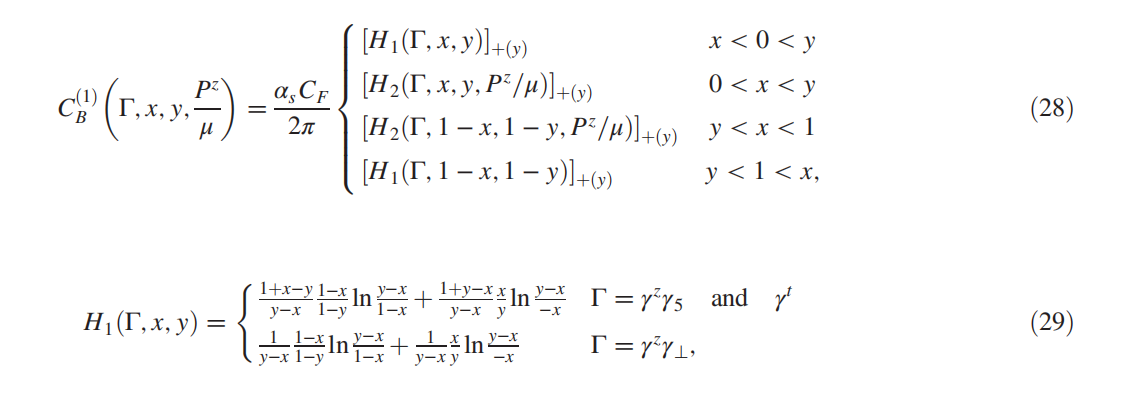
\includegraphics[scale=0.7]{fig6.png} 	
   \end{figure} 
   
     \begin{figure}
 	\centering
 	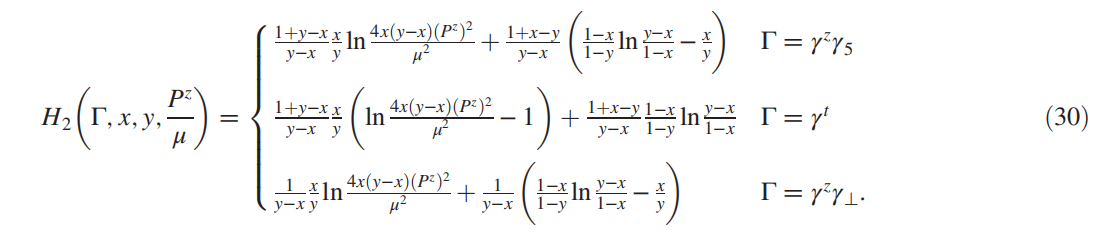
\includegraphics[scale=0.7]{fig7.png} 	
    \end{figure}  



\section{Application on lattice by Yushan Su}

\subsection{Convention}
For lattice data, $\vec{P} = (0, 0, P_z)$, $\lambda = z P_z$,

\begin{equation}
    C_2^m(z, \vec{P}, t) = \int d^3 y e^{-i \vec{P} \cdot \vec{y}} \cdot \left\langle 0\left|\bar{\psi}_{1}(\vec{y}, t) \Gamma_{1} U(\vec{y}, \vec{y}-z \hat{z}) \psi_{2}(\vec{y}-z \hat{z}, t) \cdot \bar{\psi}_{2}(0,0) \Gamma_{2} \psi_{1}(0,0)\right| 0\right\rangle
\end{equation}

\begin{equation}
    \widetilde{h}\left(\lambda, p^{z}\right)=\left.\frac{C_{2}^{m}(z, \vec{p}, t)}{C_{2}^{m}(0, \vec{p}, t)}\right|_{t \rightarrow \infty}=\frac{\left\langle 0\left|\bar{\psi}_{1}(0) \Gamma_{1} U(0,-z) \psi_{2}(-z)\right| \pi\left(p_{z}\right)\right\rangle}{\left\langle\left(0\left|\psi_{1}(0) \Gamma_{1} U(0,0) \psi_{2}  (0\right) \right| \pi\left(P_{z}\right)\right\rangle}
\end{equation}

Fourier transformation convention,

\begin{equation}
    \tilde{\phi}\left(x, p_{z}\right)=\int \frac{d \lambda}{2 \pi} e^{i \lambda x} \tilde{h}\left(\lambda, p_{z}\right)
\end{equation}

\subsection{Quasi}





\section{Inverse matching in Python}

\subsection{Matching kernel}
\begin{equation}
    \tilde{h}\left(\lambda, p_{z}\right)=\int_{0}^{\lambda} \frac{d \lambda'}{\lambda}  h(\lambda') \tilde{Z} = \int_{0}^{\lambda} d \lambda'  h(\lambda') M 
\end{equation}

\begin{equation}
    M = \delta(\lambda - \lambda') + \frac{\alpha_s C_F}{2 \pi} \delta(\lambda - \lambda') [\frac{1}{2}f(z^2, \mu^2) - \frac{3}{2}] + \frac{\alpha_s C_F}{2 \pi} [\frac{\lambda'}{\lambda - \lambda'}]_{+} \cdot \frac{1}{\lambda} [-(f(z^2, \mu^2)+1)(1+e^{-i(\lambda - \lambda')})]
\end{equation}

\begin{equation}\nonumber
    + \frac{\alpha_s C_F}{2 \pi} [\frac{\ln(1-\frac{\lambda'}{\lambda})}{1-\frac{\lambda'}{\lambda}}]_{+} \cdot \frac{1}{\lambda} [-2(1 + e^{-i(\lambda - \lambda')})] + \frac{\alpha_s C_F}{2 \pi} \frac{1- e^{-i(\lambda - \lambda')}}{i \lambda^2} (3 - f(z^2, \mu^2)) = \delta(\lambda - \lambda') + C
\end{equation}





\subsection{Method 1}
\begin{equation}
    \tilde{h}(\lambda) = h(\lambda) + \int_{0}^{\lambda} d \lambda' h(\lambda') C
\end{equation}

\begin{equation}
    h(\lambda) \approx \tilde{h}(\lambda) - \int_{0}^{\lambda} d \lambda' \tilde{h}(\lambda') C
\end{equation}

\subsubsection{How to deal with plus functions}

\noindent 

Situation 1.

\begin{equation}
    [\frac{\lambda'}{\lambda - \lambda'}]_{+} = \frac{\lambda'}{\lambda - \lambda'} - \delta(\lambda - \lambda') \int_0^{\lambda} dt \frac{t}{\lambda - t}
\end{equation}

\begin{equation}
    \tilde{f}(\lambda) = \int d \lambda' [\frac{\lambda'}{\lambda - \lambda'}]_{+} \cdot (1+e^{-i(\lambda - \lambda')}) f(\lambda') 
\end{equation}

\begin{equation}
    = \int d \lambda' [ \frac{\lambda'}{\lambda - \lambda'} (1+e^{-i(\lambda - \lambda')}) - 2 \int dt \frac{t}{\lambda - t} \delta(\lambda - \lambda') ] f(\lambda')  
\end{equation}

\begin{equation}
    = \int d \lambda' [ \frac{\lambda'}{\lambda - \lambda'} (1+e^{-i(\lambda - \lambda')}) f(\lambda') - 2 \frac{\lambda'}{\lambda - \lambda'} f(\lambda) ]
\end{equation}

Situation 2.

\begin{equation}
    [\frac{\lambda'}{\lambda - \lambda'}]_{+} = \frac{\lambda'}{\lambda - \lambda'} - \delta(\lambda - \lambda') \int_0^{+\infty} dt \frac{\lambda'}{t - \lambda'}
\end{equation}

\begin{equation}
    \tilde{f}(\lambda) = \int d \lambda' [\frac{\lambda'}{\lambda - \lambda'}]_{+} \cdot (1+e^{-i(\lambda - \lambda')}) f(\lambda') 
\end{equation}

\begin{equation}
    = \int d \lambda' \frac{\lambda'}{\lambda - \lambda'} (1+e^{-i(\lambda - \lambda')}) f(\lambda') - 2 \int_0^{+\infty} dt \frac{\lambda}{t - \lambda} f(\lambda)
\end{equation}

Here we adopt the situation 1.

\subsection{Method 2}
\begin{equation}
    \tilde{h}(\lambda) = \int_{0}^{\lambda} d \lambda'  h(\lambda') M = \bar{M} \cdot h(\lambda')
\end{equation}

\begin{equation}
    h(\lambda') = \bar{M}^{-1} \cdot \tilde{h}(\lambda)
\end{equation}

Because in the integral, $0 < \lambda' < \lambda$, our matrix $(\bar{M})_{\lambda, \lambda'}$ should be a lower triangle matrix.

\subsubsection{How to deal with plus functions}
\begin{equation}
    \tilde{f}(\lambda) = \int d \lambda' [\frac{\lambda'}{\lambda - \lambda'}]_{+} \cdot (1+e^{-i(\lambda - \lambda')}) f(\lambda') 
\end{equation}

\begin{equation}
    = \int d \lambda' [ \frac{\lambda'}{\lambda - \lambda'} (1+e^{-i(\lambda - \lambda')}) - 2 \int dt \frac{t}{\lambda - t} \delta(\lambda - \lambda') ] f(\lambda') = \int d \lambda' N f(\lambda') = \bar{N} \cdot f(\lambda')
\end{equation}

The matrix $\bar{N}$ is hard to calculate because the diagnoal elements contain two divergent terms. In order to deal with it, we integrate each lines to get some finite results, which are the summation of all elements in each lines.

\begin{equation}
    \text{Sum}(\lambda) \Delta \lambda' = \int d \lambda' N = \int d \lambda'  \frac{\lambda'}{\lambda - \lambda'} (1+e^{-i(\lambda - \lambda')})  - 2 \int dt \frac{t}{\lambda - t} = \int d \lambda'  \frac{\lambda'}{\lambda - \lambda'} (e^{-i(\lambda - \lambda')} - 1)
\end{equation}

\begin{equation}
    M_{\lambda_0 \lambda_0} = \text{Sum}(\lambda_0) - \sum_{i \neq \lambda_0} M_{\lambda_0 i}
\end{equation}

\end{document}